\documentclass[11pt,english]{article}

\setlength{\oddsidemargin}{0cm}
\setlength{\topmargin}{-2cm}
\setlength{\textwidth}{160mm}
\setlength{\textheight}{230mm}

\usepackage[english]{babel}                      
\usepackage[utf8]{inputenc}                    
\usepackage{amsmath}                             
\usepackage{amssymb}                               
\usepackage[pdftex]{graphicx}                    
\usepackage{float} 
\usepackage{subfigure} 
\usepackage[ruled,linesnumbered]{algorithm2e}
\usepackage[colorlinks, linkcolor=blue]{hyperref}
\usepackage{appendix}
\usepackage{algorithmic}
\usepackage{titletoc}
\usepackage{subcaption} % This package is used for subfigures
\usepackage{amsthm}

\newtheorem{lemma}{Lemma}
\newtheorem{definition}{Definition}

\DeclareGraphicsExtensions{.jpg,.mps,.pdf,.png}    

\usepackage{fancyhdr}

\pagestyle{fancy}
\fancyhf{} % Efface les en-têtes et pieds de page actuels
\fancyhead[C]{M1 CPA} % Texte d'en-tête
\fancyfoot[C]{\thepage}

%Sommaire en noir
\titlecontents{section}
              [0em]
              {\color{black}} % Couleur du texte
              {\bfseries\contentslabel{2.3em}}
              {\bfseries}
              {\titlerule*[1pc]{.}\bfseries\contentspage}
\hypersetup{
    colorlinks=true,
    linkcolor=black, % Couleur des liens vers des sections, sous-sections, etc.
    urlcolor=blue, % Couleur des liens URL
    citecolor=black % Couleur des liens de citation
}
\begin{document}

\title
{
    \textbf{Project CPA \\ BomberMan\\}
}

\author
{
    \\
    \\
    Submitted by
    \\
    \\
    \textbf{Haotian Xue}
    \\
    \textbf{Hejun Cao}
    \\
    M1 Science et Technologie du Logiciel 2023-2024
    \\
    Sorbonne Universite (SU UPMC)
    \\
    \\
    \\
    Under the guidance of 
    \\
    \\
    \textbf{\href{https://www-npa.lip6.fr/~buixuan/}{\textcolor{black}{Binh-Minh Bui-Xuan}}}
    \\
    Laboratoire d'Informatique de Paris 6 (LIP6)
    \\
    Centre National de la Recherche Scientifique (CNRS)
    \\
    Sorbonne Universite (SU UPMC)
}

\date{05/05/2024}

\maketitle

\begin{figure}[htbp]
    \begin{center}
        
\includegraphics[height=3cm]{./src/logo_lip6.png}
    \end{center}
\end{figure}

\begin{figure}[htbp]
    \begin{center}
        
\includegraphics[height=3cm]{./src/Science_Sorbonne_logo.png}
    \end{center}
\end{figure}

\pagebreak

\tableofcontents

\pagebreak

\large 

\section{Introduction}

\indent

Ce projet vise à utiliser Java pour implémenter les fonctions de base du jeu classique BomberMan.

\subsection{Principes du jeu}

\indent 

Une princesse est détenue prisonnière par de méchants monstres verts. Votre mission, si vous l'acceptez, est d'aller la délivrer. Pour cela, vous devrez traverser plusieurs mondes, plus effrayants les uns que les autres. Des portes vous permettront de passer de monde en monde. Certaines portes seront fermées à clé et nécessiteront d'avoir une clé dans votre inventaire. Vous êtes un expert en explosif et utiliserez vos bombes pour détruire les obstacles devant vous et tuer les monstres qui vous attaqueront.

\subsection{Représentation du jeu}

\indent

Chaque monde est représenté par une carte (rectangulaire) composée de cellules. Chaque cellule peut contenir :

-   le joueur ;

-   la princesse ;

-   des monstres ;

-   des éléments de décor (arbres, pierres...) infranchissables et
    indestructibles ;

-   des caisses destructibles et déplaçables ; 

-   des portes, ouvertes ou fermées, permettant d’évoluer entre les
    mondes ;

-   des clés pour débloquer les portes fermées ;

-   des bonus ou des malus qu'il est possible de ramasser.

\begin{figure}[H]
    \begin{center}
        \includegraphics[height=9cm]{../img/ubomb.png}
    \end{center}
\end{figure}

\subsection{ Gestion des mondes }

\indent

Nous avons chargé une configuration complète de jeu depuis un fichier. Vous trouverez un répertoire world à la racine du projet avec un fichier sample.properties représentant un monde avec 3 niveaux. Les fichiers properties en Java permettent de facilement stocker des couples de clés/valeurs.

\subsection{Mode 2 Players}

\indent

Mode deux joueurs, également un mode compétitif. Le joueur 1 utilise ZSQD ou WSAD pour se déplacer et ESPACE pour placer une bombe. Le joueur 2 utilise les flèches HAUT, BAS, GAUCHE, DROITE pour se déplacer et B pour placer une bombe.

\section {Bilan de ressource déployée}

\indent

\begin{table}[H]
    \centering
    \begin{tabular}{|p{0.45\textwidth}|p{0.45\textwidth}|}
    \hline
    Semaine1 & Déterminez le thème BombMan, créez un projet Gradle, créez des classes d'objets de fenêtre et de joueur et trouvez du matériel de jeu\\
    \hline
    Semaine2 & Ajoutez plus d'éléments au jeu, utilisez des lettres pour représenter des objets, utilisez des chaînes pour créer des cartes de jeu, utilisez des fichiers de propriétés pour charger des cartes, ajoutez un panneau d'information pour afficher le statut du joueur, ajoutez la fonction permettant aux joueurs de récupérer des accessoires et les conditions de victoire et défaite du jeu. \\
    \hline
    Semaine3 & Déverrouillez la porte et la poignée pour monter et descendre les escaliers. Utilisez un tableau pour enregistrer l'état de l'étage précédent, ce qui résout le problème des déplacements vers et depuis l'étage. Ajout de la fonction permettant aux joueurs de rendre les boîtes, et ajout initial de la fonction bombe (minuterie, les sprites de bombe changent toutes les secondes et génération de flammes d'explosion)\\
    \hline
    Semaine4 & Résolution du problème de la façon dont les flammes de l'explosion d'une bombe affectent les joueurs et d'autres objets, résolution de la logique de plusieurs bombes adjacentes explosant en même temps et ajout de changements dans les sprites qui blessaient les joueurs.\\
    \hline
    Semaine5 & Ajout d'une fonction de mouvement aléatoire et d'une fonction de mouvement directionnel des monstres \\
    \hline
    Semaine6 & Nouveaux modes ajoutés : le mode score et le mode deux joueurs génèrent aléatoirement des monstres ou des bonus à des endroits aléatoires. Le mode deux joueurs ajoute des positions clés. \\
    \hline
    Semaine7 & Ajout de la fonction de génération aléatoire de bonus après avoir bombardé une boîte, ainsi que de la musique de fond et des effets sonores du jeu. \\
    \hline
    Semaine8 & Rapport et Documentation \\
    \hline
    \end{tabular}
\end{table}
  

\section{Architecture}

\indent

L'architecture de ce projet est la suivante :

\begin{itemize}
    \item [$\bullet$] \textbf{package go}
    
    Ce package est principalement utilisé pour définir divers objets dans le jeu, notamment des personnages contrôlés par le joueur, des monstres, des arbres, des murs, des buffs/debuffs, et bien plus encore.
    
    En même temps, il définit également les actions individuelles du joueur/monstre. 

    Pour les joueurs, nous avons conçu son jugement de mouvement (s'il peut se déplacer dans la direction indiquée), la récupération des buffs/débuffs et la prévention des bombes.

    Pour les buffs et debuffs, nous avons mis en place une augmentation/diminution du nombre de bombes ou de la portée d'explosion.

    \item [$\bullet$] \textbf{package game}
    
    Ce package est principalement utilisé pour localiser les joueurs et les monstres, et calculer la prochaine position du joueur/monstre, ainsi que le niveau de difficulté actuel.

    \item [$\bullet$] \textbf{package engine}
    
    Il s'agit du package principal qui pilote l'implémentation du jeu. Il implémente principalement le cycle de vie de l’ensemble du jeu. Il est chargé de rafraîchir constamment tout l'écran de jeu, de charger et de mettre en œuvre l'animation (Sprite) correspondant à chaque élément, le mouvement automatique des monstres et la prédiction d'action correspondante (où apparaîtra la prochaine image).

    \item [$\bullet$] \textbf{package launcher}
    
    Ce package est principalement utilisé pour définir des cartes par défaut et charger de nouvelles cartes.

    \item [$\bullet$] \textbf{package view/audio}
    
    Ces deux packages sont principalement utilisés pour charger des images et des sons.
    

\end{itemize}

\indent Le cycle de vie principal du jeu est le suivant :

\begin{figure}[H]
    \begin{center}
        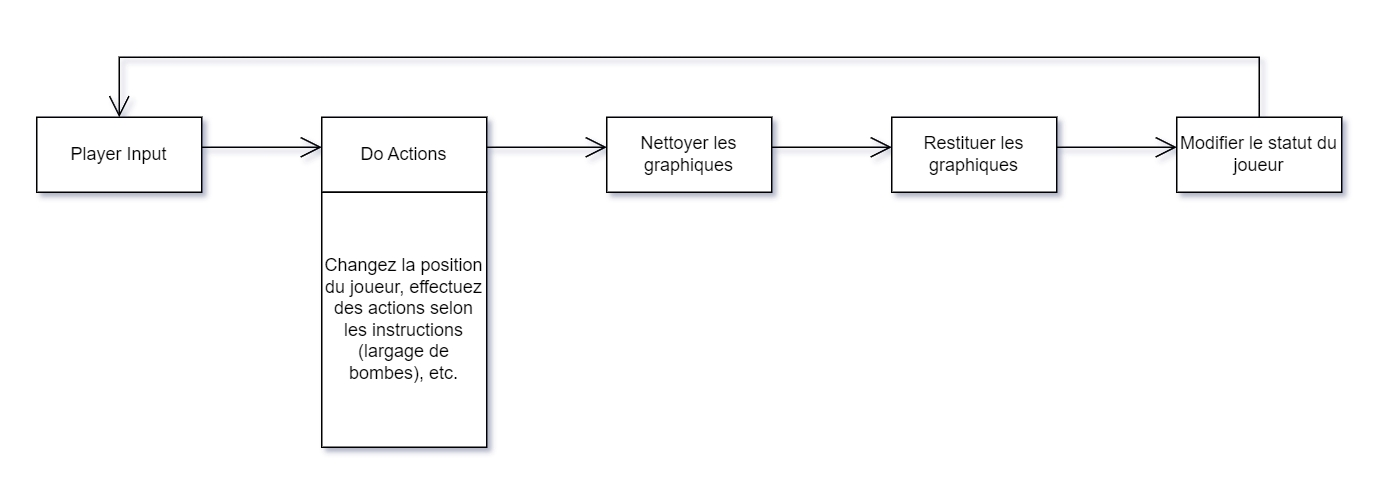
\includegraphics[height=5.5cm]{./src/cycle.png}
    \end{center}
\end{figure}

\indent De plus, j'ai dessiné le diagramme UML suivant :

\begin{figure}[H]
    \begin{center}
        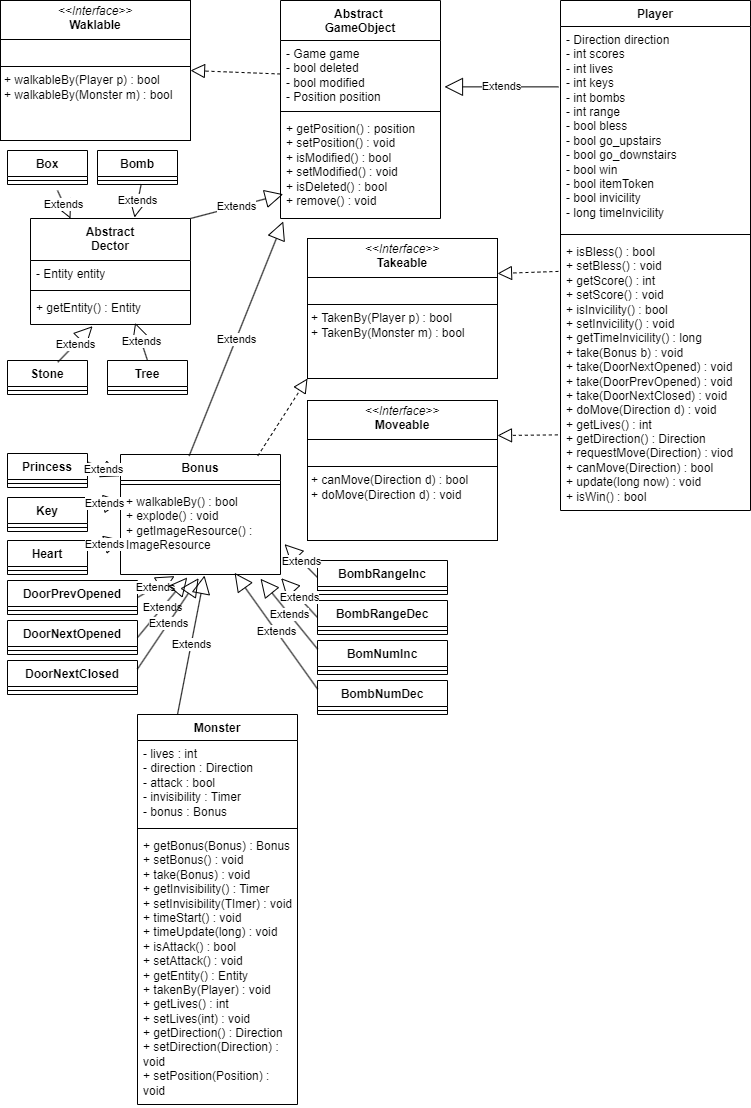
\includegraphics[height = 21cm]{./src/UML_Class.png}
    \end{center}
\end{figure}

\pagebreak

\section{Présentation Visuelle}

\indent

Nous chargeons les images de chaque objet via la classe SpriteFactory. 

\indent Pour les joueurs et les monstres, il y a des images correspondant à quatre directions. 

\begin{figure}[H]  
    \centering
    \subfigure[]{
    \begin{minipage}[b]{0.2\textwidth}
    
\includegraphics[width=1\textwidth]{../src/main/resources/images/player_left.png} \\
    
\includegraphics[width=1\textwidth]{../src/main/resources/images/player_right.png}
    \end{minipage}
    }
    \subfigure[]{
    \begin{minipage}[b]{0.2\textwidth}
    
\includegraphics[width=1\textwidth]{../src/main/resources/images/player_up.png} \\
    
\includegraphics[width=1\textwidth]{../src/main/resources/images/player_down.png}
    \end{minipage}
    }
\end{figure}
    
\indent Pour une bombe, la longueur de sa mèche changera avec le temps et elle explosera après avoir atteint 4 secondes.

\begin{figure}[H]  
    \centering
    \subfigure[]{
    \begin{minipage}[b]{0.2\textwidth}
    
\includegraphics[width=1\textwidth]{../src/main/resources/images/bomb_3.png} \\
    
\includegraphics[width=1\textwidth]{../src/main/resources/images/bomb_1.png}
    \end{minipage}
    }
    \subfigure[]{
    \begin{minipage}[b]{0.2\textwidth}
    
\includegraphics[width=1\textwidth]{../src/main/resources/images/bomb_2.png} \\
    
\includegraphics[width=1\textwidth]{../src/main/resources/images/bomb_0.png}
    \end{minipage}
    }
    \subfigure[]{
        \begin{minipage}[b]{0.2\textwidth}
        
\includegraphics[width=1\textwidth]{../src/main/resources/images/explosion.png}
        \end{minipage}
    }
\end{figure}

\indent De plus, lorsque le joueur entre dans la zone d'attaque du monstre, un point d'exclamation apparaîtra sur la tête du monstre.

\begin{figure}[H]  
    \centering
    \subfigure[]{
    \begin{minipage}[b]{0.2\textwidth}
    
\includegraphics[width=1\textwidth]{../src/main/resources/images/monster_attack_left.png} \\
    
\includegraphics[width=1\textwidth]{../src/main/resources/images/monster_attack_right.png}
    \end{minipage}
    }
    \subfigure[]{
    \begin{minipage}[b]{0.2\textwidth}
    
\includegraphics[width=1\textwidth]{../src/main/resources/images/monster_attack_up.png} \\
    
\includegraphics[width=1\textwidth]{../src/main/resources/images/monster_attack_down.png}
    \end{minipage}
    }
\end{figure}

\indent Selon le cycle de vie du jeu donné précédemment, chaque fois que nous calculons l'état correspondant à chaque objet dans l'image suivante, nous mettrons à jour l'écran et remplacerons les images de tous les objets modifiés.

\section{Algorithme}

\subsection{Map Compression/Decompression}

\indent

Notre carte est en fait éditée dans un format de tableau bidimensionnel, ce qui entraînera de très sérieux problèmes de stockage car les éléments de notre carte ne sont pas très complexes et comportent de nombreux objets en double.

\indent Afin d'optimiser ce problème, nous avons conçu un algorithme de compression et de décompression pour les cartes afin de stocker et de transmettre les informations cartographiques plus efficacement.

\indent La logique de la compression de carte est la suivante :

\small
{
\begin{itemize}
    \item [$\bullet$] \textit{Step 1}
    
    Comme je l'ai dit précédemment, la carte est stockée sous la forme d'un tableau à deux dimensions. Nous parcourons donc les éléments de la carte ligne par ligne et obtenons le codage des caractères de chaque élément (via la fonction getCode), puis nous ajoutons tous ces codages à une chaîne de caractères.

    \item [$\bullet$] \textit{Step 2}
    
    Chaque fois que nous finissons de parcourir une ligne de données, nous ajoutons un "x" pour indiquer une nouvelle ligne.

    \item [$\bullet$] \textit{Step 3}
    
    Par la suite, nous utilisons un simple algorithme RLE (Run-Length Encoding) pour modifier les éléments répétés consécutifs sous forme de nombres + encodage. Par exemple, TTT (représentant trois arbres consécutifs) sera converti en 3T.

\end{itemize}
}

\large

Pour la partie décompression, c’est en fait l’inverse complet du processus de compression. Tout d'abord, la chaîne après RLE est traitée et restaurée sous la forme où un seul objet occupe un caractère, puis, sur la base du caractère de nouvelle ligne "x", le tableau bidimensionnel correspondant à la carte est construit ligne par ligne.


\subsection{IA pour Monstres}

\indent 

Dans n'importe quel jeu, les actions de l'IA de l'ennemi jouent un rôle très important, c'est pourquoi leurs algorithmes d'IA sont particulièrement importants.

\indent Puisque la seule interaction entre les monstres et les joueurs dans notre jeu est le jugement de position, la partie la plus importante est en fait la logique de recherche de chemin du monstre, qui consiste à trouver le chemin le plus court vers l'emplacement actuel du joueur.

\indent Nous avons d'abord conçu une plage de haine pour chaque monstre. Le mécanisme de recherche de chemin du monstre sera déclenché lorsque et seulement lorsque le joueur apparaîtra dans cette plage. À d'autres moments, le monstre se déplacera de manière aléatoire dans n'importe quelle direction.

\indent Quant à la recherche active du monstre, nous avons choisi l'algorithme heuristique au lieu de l'algorithme A-star, Parce que notre carte est petite, l'avantage de vitesse de l'algorithme A-star n'est pas évident. Par rapport à la simplicité de l'algorithme de recherche heuristique, l'algorithme A-star est plus difficile à mettre en œuvre.

\indent Notre conception heuristique est très simple :

\small
{
\begin{itemize}
    \item [$\bullet$] \textit{Regle 1}
    
    Si le monstre est différent du joueur sur l'axe des x, déplacez l'axe des x du monstre pour qu'il se déplace vers le joueur.

    \item [$\bullet$] \textit{Regle 2}
    
    S'il y a une différence sur l'axe y entre le monstre et le joueur, déplacez l'axe y du monstre pour qu'il se déplace vers le joueur.

    \item [$\bullet$] \textit{Regle 3}
    
    Donnez la priorité au déplacement de l’axe x du monstre.

\end{itemize}
}

\large

\indent Cependant, une telle heuristique pose toujours un problème : si le monstre se retrouve dans une impasse, il y attendra au lieu d’essayer d’autres chemins.

\subsection{Move Test}

\indent 

Dans la première version de ce projet, même si nous avions correctement ajouté la détection de collision entre le joueur (monstre) et l'objet, il y avait encore des scènes fréquentes où le joueur (monstre) restait coincé dans le mur et était incapable de bouger.

\indent Après de nombreux tests, nous avons constaté que les personnages qui changent de position en synchronisation avec nos pressions sur les boutons, en raison de l'étirement du temps, se déplacent en fait plus loin que prévu, ce qui peut entraîner des problèmes avec les personnages qui restent coincés dans les murs.

\indent Notre solution consiste à préjuger le mouvement des joueurs et des monstres. C'est-à-dire que nous devons d'abord déterminer si sa position dans l'image suivante est raisonnable avant qu'il ne bouge réellement, au lieu de modifier directement ses informations de position, puis de déterminer si le mouvement est réel. l'emplacement est raisonnable.

\section{Gestion de Collisions}

\indent 

Gestion unifiée des erreurs : établissez un cadre global de gestion des exceptions pour capturer et répondre aux exceptions d'exécution dans le jeu.

\indent Journalisation détaillée : implémentez un système de journalisation pour enregistrer les opérations des utilisateurs et les erreurs système afin de faciliter le débogage et l'analyse.

\indent Nous utilisons des frameworks de journalisation tels que Log4j ou SLF4J pour mettre en œuvre des stratégies de journalisation détaillées. Ajoutez la journalisation aux points opérationnels clés, tels que la lecture et l’écriture de fichiers et les opérations utilisateur importantes.

\section{Conclusion}

\indent

Ce projet vise à développer un remake 2D du jeu classique appelé BomberMan. Le gameplay principal du jeu consiste à placer des bombes pour détruire les ennemis et détruire les obstacles tout en évitant d'être affecté par les explosions de bombes. Le projet est développé en langage Java et utilise la technologie Sprite pour obtenir des graphismes de jeu dynamiques.

\indent En termes de mise en œuvre technique, ce projet exploite pleinement les capacités de programmation orientée objet de Java en concevant des structures de classes détaillées pour gérer diverses entités du jeu, telles que les joueurs, les bombes, les monstres et les obstacles. Les sprites sont utilisés pour créer des animations fluides et répondre aux interactions des utilisateurs, améliorant ainsi les visuels du jeu.

\indent L’un des principaux défis techniques auxquels nous avons été confrontés consistait à mettre en œuvre une logique de détection de collision efficace, qui a finalement été résolue par la prédiction des actions.

\indent Grâce à ce projet, nous avons appris en profondeur divers aspects de la programmation Java et de la conception de jeux. J'ai notamment acquis une expérience précieuse dans l'optimisation des performances des jeux et la gestion des ressources. La résolution des problèmes rencontrés lors de la détection de collisions et de la mise en œuvre d'animations m'a permis de mieux comprendre la programmation événementielle.

\end{document}